\documentclass[11pt]{book}
\usepackage[margin=1in]{geometry}
\usepackage[T1]{fontenc}
\usepackage[utf8]{inputenc}
\usepackage{lmodern}
\usepackage[hidelinks]{hyperref}
\usepackage{amsmath,amssymb}

\makeatletter
\@addtoreset{chapter}{part}
\makeatother

\renewcommand{\thepart}{\Roman{part}}
\renewcommand{\thechapter}{\arabic{chapter}}

\setlength{\parindent}{1em}
\setlength{\parskip}{0pt}


\begin{document}

\title{Everything I Learned}
\author{Jacob K. Davis}
\date{\today}
\maketitle

\section{What is this book?}
This is a book of everything that I've learned throughout my college journey; from taking
prerequisites all the way to the final course before graduation.
\subsection{Why?}
Over 4 years, I have accrued over \$30 thousand dollars in debt, had many sleepless nights,
went through a break-up (probably in part due to school), and struggled financially for most of it.
Beyond just a piece of paper I paid a lot of money for, I figured what better way
to visually see everything I've gone through?

Actually, I'm somewhat lying, the
idea came from a book that I read called
\textit{"Surely You're Joking, Mr. Feynman!"} Adventures of a Curious Character%
\footnote{Richard P. Feynman and Ralph Leighton,
\textit{“Surely You're Joking, Mr. Feynman!”: Adventures of a Curious Character},
W. W. Norton \& Company, 1985.}. Well, technically not from the actual book, but
from the guy who wrote it, Dr. Richard Feynman. There is a quote by him that reads
"What I cannot create, I do not understand" and from it, the Feynman Technique was created.

The idea is simple: \textbf{if you can’t explain something to a five-year-old, you don’t really understand it.}
So, dear reader—you are my five-year-olds. I hope you understand everything I’m about to say.

As I write this, it is October 20th, 2025 - 4-ish years since I took that first
College Algebra course. Since I am starting this so late, this means I have to
chase down old notes, decipher my god awful handwriting, and try to put it into
words that actually make sense. Because of this, there will inevitably be large
chunks of courses missing. That's okay, because this isn't as much about the content,
but my journey through it.


\subsection{Who is this for?}
I don't know, maybe no one. It's not an attempt to tell a story, it's to share my
experiences. This means that there could be sections that should be read by family,
sections that should be read by professors, or maybe even sections I should re-read.
I don't ever plan on selling this, maybe just making a few copies to give to those
that mean the most to me. If you're reading this, you've probably stumbled upon it
at a yard sale, or you're one of those people who mean the most to me. I did pay
to get this made with my hard-earned Computer Science degree, you know.

\subsubsection{For my Mom}
Since it seems to be an "unwritten rule" to dedicate a book to someone, I dedicate
this to my Mom. On April 18, 2021, she watched her only son leave to travel 1,688 miles
away to Austin, Texas. She never told me no or that I should think about it; she actually
encouraged me to go. She knew that I wouldn't go otherwise.

I know that it crushed her,
but I think she knew deep down that this is what I needed. Since then, she has spent countless
hours on the phone with me listening to me vent about school. She has been my rock and
will forever be the reason I am the person I am today.

I am grateful for her beyond just school, but for everything that I have accomplished
because of it. Without her, I would never have left. So yeah, I think that she deserves
more than just a paragraph in a book of MY life.


\tableofcontents


\part{Computer Science}
\chapter{Fundamentals of CS}

This is some text i added to see if it works
\chapter{Programming Fundamentals II}
\chapter{Foundations of CS II}
\chapter{Assembly Language}
\chapter{Computer Ethics}
\chapter{Data Structures and Algorithms}
\chapter{Object-Oriented Design and Programming}
\chapter{Software Engineering}

I took this class in the Fall of 2025 with a professor named Dr. Lehr. Several students have described his personality as “Jekyll and Hyde,” and while I wholeheartedly agree, I’d add that his grading fits the same description.

That said, this course may be one of the most practical and applicable in my entire Computer Science degree. Why? Because it’s designed to simulate a real working environment. The class was divided into groups of three to five members, and each team was tasked with creating a project. My group decided to build a
\textbf{Music Recommendation App.}

The project was written in React and Python — React for the frontend, and Python for the backend. I spent most of my time working on the backend.

If you’re reading this and thinking, “What the heck is a frontend or backend?” here’s a quick explanation: the frontend is what you see; the backend is what makes what you see work. Think of Facebook — when you scroll through your newsfeed and see everyone posting cute cat photos or ranting about the latest political crisis, the frontend is what’s displayed on the screen. The backend is where all that content lives, stored in a massive database. Every post, comment, and like is just a piece of data among billions of others.

If you’re curious about how that data gets from Facebook’s servers to your screen in the blink of an eye, check out my notes on \textbf{Data Structures and Algorithms.}


\section{Music Recommendation App}
\subsection{The Idea Behind It}


\chapter{Computer System Security}
I took this class in the Fall of 2025 with a notably "poor" professor named
Randall "Randy" Klepetko and let me tell you... I really need to stop reading the reviews
about professors on RateMyProfessor because he was anything but "poor". To paint a picture
of Dr. Klepetko, go to a Grateful Dead concert and pick any long haired, maybe late fifty's,
tall skinny dude out of the crowd, and I'd say they might be a spitting image of him. I mean
this in the absolute best way possible; he literally would be at that concert, and it may
very much be him. The reviews said things along the lines of "he's rude to students", or
"his tests are impossible". While I've never heard him be rude to a student, I can say that
the tests were inherently challenging due to the nature of the courses he taught (this one and
Computer Architecture). So main takeaway from this course? Don't believe what you read on the
internet, especially if it's written by a frustrated 18-year-old who couldn't ChatGPT their
way through the course.

So what is this course? It's a very high level of understanding what Computer System Security
is and understanding some of the threats that machines (computers) are exposed to.

\section{Introduction}
\section{Attacks}
\section{Defenses}
What is more challenging; Attacking or Defending a computer? Defending, by far.
To attack a computer, you only need to find one vulnerability; To defend one, you
have to mitigate all vulnerabilities.



\subsection{Monitoring/Detection}
In order to prevent attacks, a system must continuously monitor changes to detect
any potential threats. The system monitors:

\begin{itemize}
    \item Files
    \item Memory
    \item Processes
    \item Input/Output
    \item Disk Activity
\end{itemize}


Each is monitored by two different types of Detection Analysis

\subsubsection{Static Analysis}

\textbf{Static Analysis} is your \textbf{Anti-Virus} or \textbf{file alteration
detection} software. It constantly checks whether there is a \textit{"virus
file"} present on the machine. If one is detected, it immediately puts it into
quarantine to prevent it from making any unauthorized changes. Antivirus
software is \textbf{very effective}, almost 99\% percent of the time it can pick
up these types of files.

I would assume that it's so effective because it has seen thousands and
thousands of different iterations of all the possible file constructs to be able
to detect whether a file is safe. Because of this, Antivirus is ineffective
against \textit{Zero-Day Exploits} \newline

\begin{tcolorbox}[mybox] A \textbf{\textit{Zero-Day Exploit}} is a type of
attack that attempts to inject itself into a brand-new program before the first
patch is released.


\begin{center} 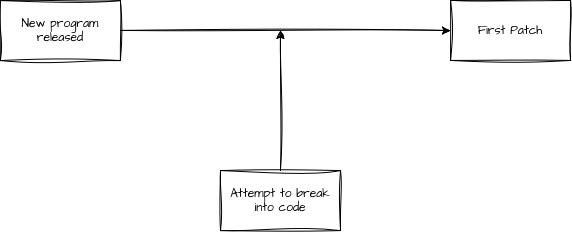
\includegraphics[width=400px]{zero_day} \end{center}

\end{tcolorbox}

\subsubsection{Dynamic Analysis} \textbf{Dynamic Analysis} dynamically checks
whether certain events fall meet a certain set of criteria  of a specified
range, using either the Poisson or Gaussian Distribution. For example, it could
be the number of times a file tries to access a directory whose permissions are
locked. If it tries, say, 100 times, then that would appear as an outlier on
either distribution.  Once this happens, it then quarantines the file to make
sure that if it is indeed a virus, it can't do any more damage.


Because it is running on live \textit{(dynamic data)}, it is not as effective as
Static Analysis because it's "learning as it goes", sort of. While it's not good
as a first line of defense, it's fantastic at detecting \textit{Zero-Day
Exploits.}

\subsubsection{Specification Anomalies}


\subsubsection{Machine Learning}
Machine Learning is used to detect different anomalies.
\subsection{Response and Recovery}
What is the proper course of action when, through either Static or Dynamic Analysis,
to take when a questionable file is detected?

\begin{enumerate}
    \item \textbf{Document} the attack. What happened, where did it come from, etc.
    \item \textbf{Disconnect and Delay}. Try to disconnect the part of the system that caused the attack. If say, the Hard Disk Drive is detected as the source, electronically disconnect that from the rest of the system.
    \item \textbf{Monitor} the system for any further anomalies. I would think that this is a type of monitoring that is on steroids.
    \item \textbf{Isolate} the file/root of the attack and put it's ass in jail. Not literally, but quarantine it so that it can't cause any more damage.
    \item \textbf{Set up a Honeypot} to see if there are any more sneaky bastards hanging around that weren't detected.
    \item \textbf{Misdirect} or set up a trap door for those attacks.
    \item \textbf{Restore and Recover} files that were damaged to an earlier restore point, if possible. Otherwise, tell the user they are silly goose's for not backing up their system and then proceed throw errors.
\end{enumerate}

\begin{tcolorbox}[mybox]
A good procedure to follow is called the \textbf{LOCUS Approach}. The fundamental ideas are
\begin{center}
    \textbf{Establish a security foundation} and \textbf{implement best practice standards.}
\end{center}

\end{tcolorbox}




\part{Mathematics}
\chapter{College Algebra}
\chapter{Pre-Calculus Functions and Graphs}
\chapter{Calculus I: Differential Calculus}
\chapter{Calculus II: Integral Calculus}
This was one of the most challenging courses throughout school. It was challenging
because Integral's take no prisoners. I mean, there is literally a book that has
thousands of solutions to integrals that a human brain can't solve without a computer.


Many say that this was a "weed-out" course for aspiring computer scientists, but I digress.
This course was hard because it required me to push myself to do "just one more integral" when
I didn't want to see that hideous \(\int\) sign again.




\section{How it ended}
This was actually the first class that I got a C in. This was also the first class that
I was happy to get a C in.
\chapter{Discrete Math}
\chapter{Introduction to Probability and Statistics}
\chapter{Advanced Probability and Statistics}
\chapter{Linear Algebra}
I took this course in the Fall of 2024. That semester was a pretty low point for me mentally. Not
because of the course, but personal reasons. I was over school.


\section{Matrix Algebra and Systems of Linear Equations}
To understand what Matrix Algebra is, I have to make sure you understand what
a System of Linear Equations is. Thankfully, this is pretty straight forward.

\subsection{Systems of Linear Equations}
A system of Linear Equations is more than one Linear Equation

\begin{tcolorbox}[mybox]
    \textbf{Recall: } A \textit{Linear Equation} is an equation in the form
    \(a_1x_1 + \dots + a_{n} x_{n} +b = 0\), where \(x_1, \dots, x_{n}\) are the
    \textbf{variables} and \(b, a_1, \dots, a_n\) are the \textbf{coefficients}


    \vspace{1\baselineskip}

    If you forgot what a coefficient was, it's a number that doesn't change. e.g.
    \(\pi x^2 + 3x + 9\). \(\pi, 2\) and \(9\) are the coefficients.

    \vspace{1\baselineskip}

    And, you're killing me, if you forgot what a \textbf{variable} was: it's the
    number that DOES change. In the above example, the \(x\)'s are the variables.
\end{tcolorbox}


\begin{tcolorbox}[important]
     A linear equation can not have combined variables, for example:
    \begin{equation}
        3x_{1}x_{2} + x_{3} = 10
    \end{equation}
    is \textbf{invalid}
\end{tcolorbox}
So a system of Linear Equations is more than one of those, which we stack up into a matrix.
Boom, killed two birds with one stone there.

Consider the two equations \(2x^2 + 3x - 1 \) and \(9x^2 + x\), represented in matrix form
we have:
\begin{equation}
\begin{bmatrix}
    2x^2 + 3x - 1 \\
    9x^2 + x
\end{bmatrix}
\end{equation}

This leads to the next topic,
\subsection{Ways to represent Systems of Linear Equations}
Let's take the equation used in the above example. We can represent this in two ways:

\subsubsection{Coefficient Matrix}
The first way a \textbf{coefficients' matrix} is a matrix that is just the coefficients
of the problem, so we have:
\begin{equation}
    \begin{bmatrix}
        2 & 3 & -1 \\
        9 & 1 & 0
    \end{bmatrix}
\end{equation}

The -1 represents the \(-1x^0\) from the first equation and since there is none
in the second, it's replaced with \(0 x^0\)

\subsubsection{Adjacency Matrix}
Similarly, an Adjacency Matrix includes the solution, or \(b\). We use this more since
it's got some cool stuff going on and answers some important questions, but more on that
later. For right now, let's just show what it looks like:
\begin{equation}
    \begin{bmatrix}
        2 & 3 & -1 & b_1 \\
        9 & 1 & 0 & b_2
    \end{bmatrix}
\end{equation}


\subsubsection{now what?}

Okay, so now what? Well, first, maybe it's important to understand why we use
systems of linear equations and all of these fancy shmancy formats.

Say you have \$20.00 and you have to go out and buy some milk and a soda. You get to the store and
see that a gallon of milk is \$2.75 and a soda is \$2.50. You notice that the milk is on sale, so you want to see how many you can buy. Being the little math wizz you are, you come up with the equation
\begin{equation}
    \begin{split}
    2.75x + 2.50 &= 20.00 \\
    2.75x &= 17.25 \\
    x & \approx 6.27 \text{ gallons of milk}
    \end{split}
\end{equation}
but what happens if your Mom calls you and says OJ is on sale too, get as much as you can!
Well, now you have a problem, because you want to find the most amount of OJ (valued at \$1.25) and the most amount
of milk you can get with \$20.00. Insert Linear freakin' algebra.

You now have 2 equations you can put together.
\begin{equation}
    \begin{split}
        2.75x + 2.50 &= 20.00, \\
        2.75x + 1.25y &= 20.00.
    \end{split}
\end{equation}

You can try to solve this, and sure, it's not impossible, but what if I told you that
there was a much, much easier way to do this? Well, you have no choice, you can solve it yourself,
close and close this book, or you can see the better way.

\section{Row Reduction}
(Don't worry, we will solve the OJ problem (no, not whether the glove fit, Orange Juice)),


\section{Vector Spaces and Subspaces}
\subsection{Vector Spaces}
Vector Spaces are the areas (spaces) where vectors can "live", based on predefined parameters that can be \textit{added} and \textit{scaled} while satisfying 10 properties listed in the book (The important ones are listed.). If we think of a vector space say, H = \( \left\{ \begin{bmatrix} x \\ y \end{bmatrix}  : x \geq 0, y \geq 0 \right\} \in \mathbb{R}^2 \gets\) says \textit{A vector} \(x\) and \(y\) \textit{should be greater than 0 for both values, and would therefore fall in that vector space.} On a Cartesian plane (I swear, if you need to ask what this is), it would look something like this:
\begin{center} 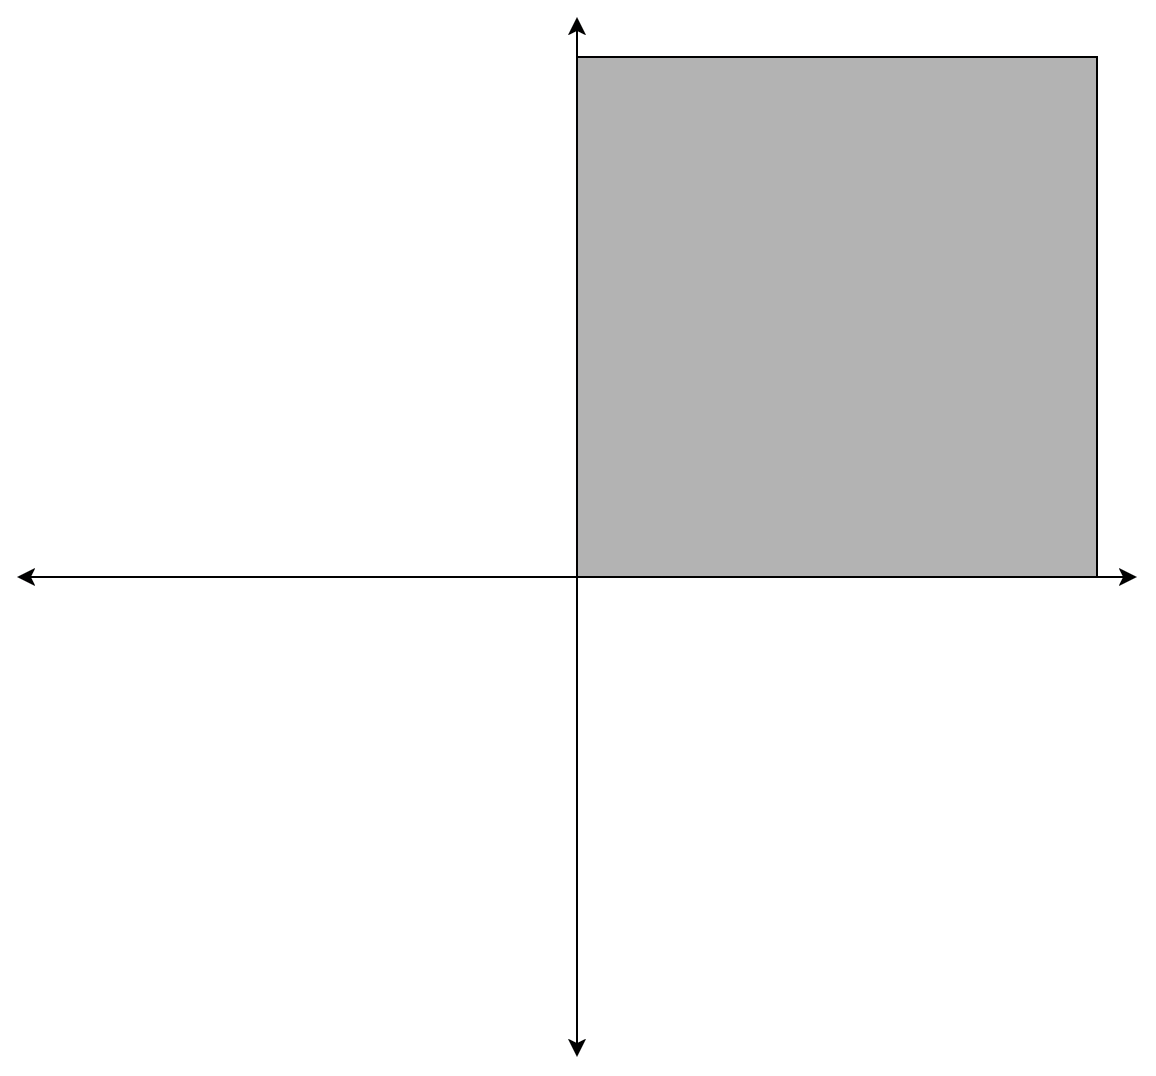
\includegraphics[width=200px]{8.3_vec_spaces.png} \end{center}
This then must satisfy 10 different properties (found in the text book, but I am only going to explain the 3 that we said to be the most useful. You can look up the other 7 if you have to.)
\begin{enumerate}
    \item The vector being tested must satisfy the \textbf{zero vector}.
    \item It must be \textbf{closed under addition} (In this example, it must be in \(\mathbb{R}^2\))
    \item It must be \textbf{closed under multiplication}. (Same thing, must be in \(\mathbb{R}^2\))
\end{enumerate}

\begin{tcolorbox}[mybox]
    In simplest terms, this just means that \(\vec{v} + \vec{w}\) and \(c\vec{w}\) must \textbf{stay in the set.}
\end{tcolorbox}

Now, lets do some actual math, shall we? Let us use the same example as above, \( \left\{ \begin{bmatrix} x \\ y \end{bmatrix}  : x \geq 0, y \geq 0 \right\} \in \mathbb{R}^2 \) and we have two vectors: \(\vec{w} = \begin{bmatrix} 2 \\ 1 \end{bmatrix}\) and \(\vec{u} = \begin{bmatrix} 1 \\ 1 \end{bmatrix}\).




\begin{center} 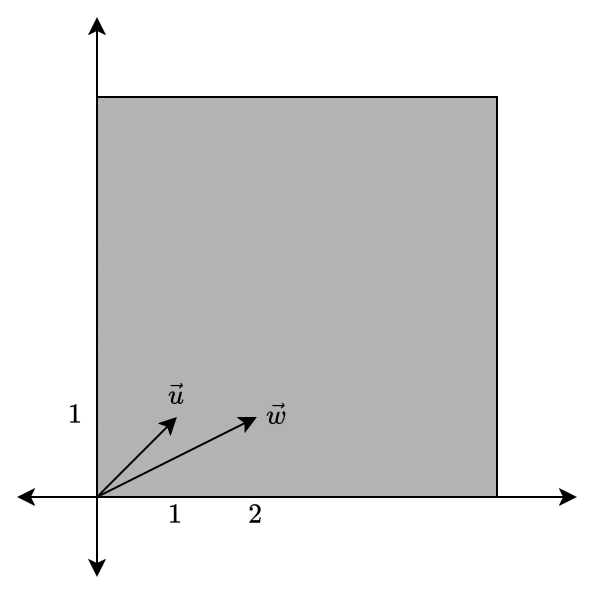
\includegraphics[width=200px]{8.3_vec_spaces_2.png} \end{center}
\subsection{Subspaces}
\textbf{Subspaces} are spaces in a \textit{vector space}. It's really just a more restricted area of the entire vector space that is being tested against. For example, when it says a vector that is in \(\mathbb{P}_n\), it's saying \textit{ a vector that is in the \textbf{BIGGER} set of } \(\mathbb{P}_n\)

\part{Physics}
\chapter{General Physics I}


\part{History}
\chapter{US History to 1877}
\chapter{US History to Date}
\chapter{Principles of American Government}
\chapter{Functions of American Government}

\part{Electives}
\chapter{Stellar Astronomy}
\chapter{Introduction to Philosophy}
\chapter{Fundamentals of Human Communication}
\chapter{Technical Writing}
\chapter{Introduction to Fine Arts}


\part{Language}
\chapter{Spanish I}

\part{Experiences}
\chapter{What Went Right}

This title is pretty self-explanatory, no? Here I log what went wrong in my journey
and my attempt at understanding why.

\section{Group Projects}
Yup. Not working in them, but the quality of students that school had. Every single
group project that I was a part of, there was one or two students who showed up at
10pm the night of the deadline to make sure their name was on the paper so they could get
the grade.
\end{document}

